\item \points{1bi} {\bf Run Fine-Tuning}

Run the command:
    
{\small\texttt{python3 main.py --task run\_ft --model bert-tiny,bert-med --dataset amazon --k 1,8,128}}

to fine-tune two sizes of BERT models on the Amazon Reviews dataset for various values of $k$. While debugging, you can pass only one value for each of the arguments to run only that subset, e.g. \texttt{python3 main.py --task run\_ft --model bert-tiny --dataset amazon --k 1}.

If you see a log message like \texttt{Some weights of the model checkpoint...}, this is expected, since the pre-trained model does not contain a prediction head for our task (this is why we need to fine-tune!).

To plot your results, run the command:

{\small\texttt{python3 main.py --task plot\_ft --model bert-tiny,bert-med --dataset amazon --k 1,8,128}}

Your plot should look as follows:
\begin{figure}[H]
    \centering
    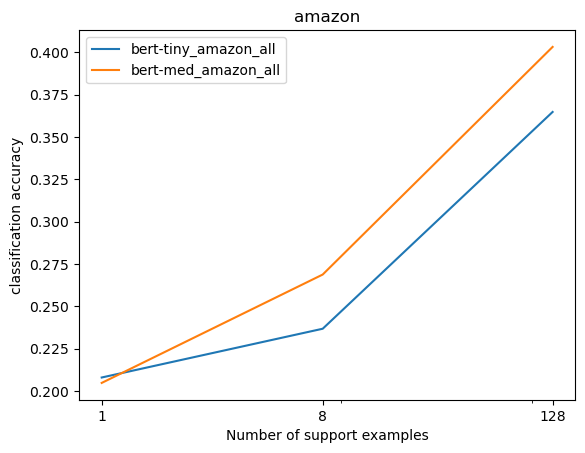
\includegraphics[width=0.75\linewidth]{./figures/q1_plot}
    \caption{Performance of two sizes of BERT models on the Amazon Reviews dataset for various values of \textit{k}}
\end{figure}

\clearpage
